\begin{refsection}[research/maruyama/group.bib]
\nocite{*}
\chapter{HPC Programming Framework Research Team}

\section{Members}

\begin{itemize}
  \item[] Naoya Maruyama (Team Leader)
  \item[] Motohiko Matsuda (Research Scientist)
  \item[] Shinichiro Takizawa (Research Scientist)
  \item[] Mohamed Wahib (Postdoctoral Researcher)
  \item[] Keisuke Fukuda (Research Associate)
  \item[] Koji Ueno (Student Trainee)
  \item[] An Huynh (Student Trainee)
  \item[] Satoshi Matsuoka (Senior Visiting Scientist)
  \item[] Tomoko Nakashima (Assistant)
  \item[] Aya Motohashi (Assistant)
\end{itemize}

Text for research Results and achievements. Journal-artcile~\cite{sample-journal}.
Conference-paper~\cite{sample-conference}.
Invited-talk~\cite{sample-invited}.

For cross referencing, use \verb|\locallabel| and \verb|\localref| to avoid conflicting names defined by other groups. For example, a figure can be referenced as Figure~\localref{fig:sample-label1}.

\begin{figure}
\centering
  
\includegraphics[width=0.5\textwidth,keepaspectratio,natwidth=193,natheight=40]
  {sample_division/sample_group/test1.png}
  \caption{Caption for a sample figure}
  \locallabel{fig:sample-label1}
\end{figure}

\section{Research Activities}

We develop high performance, highly productive software stacks that aim to simplify development of highly optimized, fault-tolerant computational science applications on current and future supercomputers, notably the K computer. Our current focus of work includes large-scale data processing, heterogeneous computing, and fault tolerance. A major ongoing project in our group will deliver a MapReduce runtime that is highly optimized for the intra- and inter-node architectures of the K computer as well as its peta-scale hierarchical storage systems. Another major project focuses on performance and productivity in large-scale heterogeneous systems. We also study high performance graph analytics on the K computer. Below is a brief summary of each project.

\section{Research Results and Achievements}

\subsection{KMR}
% Takizawa & Matsuda
\subsubsection{Improve locality when running MPI programs as MapReduce tasks}

Although MapReduce systems can allocate tasks to nodes where their inputs reside to increase data locality for improving performance, these systems only target on tasks implemented as serial programs and do not consider running tasks implemented as parallel programs using MPI as Map or Reduce task.
As many scientific applications are implemented using MPI and some application workflows form ensemble execution patterns of such MPI programs, the workflows can be implemented easily and efficient data access can be achieved if a MapReduce system can allocate tasks implemented using MPI so that it can exploit data locality in them.

We proposed an extension of the execution model of MapReduce to achieve high performance when running MPI programs as Map/Reduce tasks.
We model data to be processed as Key-Value as the traditional MapReduce model.
However, to processing the data, we propose a new \verb|map| function which makes process groups where each process in a group has a key-value whose key is same as those of other processes in the group and applies a user-defined mapper, which is implemented using MPI, to the key-values using processes in each group.

\begin{figure}
\centering
  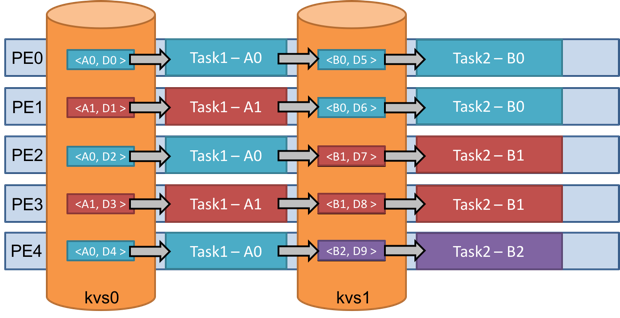
\includegraphics[width=0.5\textwidth,keepaspectratio,natwidth=193,natheight=40]
  {research/maruyama/lo01.png}
%  \caption{Caption for a sample figure}
  \locallabel{fig:kmr-01}
\end{figure}

To evaluate our proposal, we used $N \times N$ nodes of the K computer and compared performance of our method in which data access was performed locally and that of random data access.
We used a synthetic benchmark program where each node has an individual data and which iterates the following two computation; the first computation groups $N$ nodes in low direction and processes data on them, and the second groups $N$ nodes in column direction and processes data on them.
The result is shown in the figure.
The horizontal axis is the amount of data on each node and the virtical axis is the relative performance of an iteration against random data access.
As can be seen from the figure, the performance of our proposal improve as the number of nodes and the amount of data increase.

\begin{figure}
\centering
  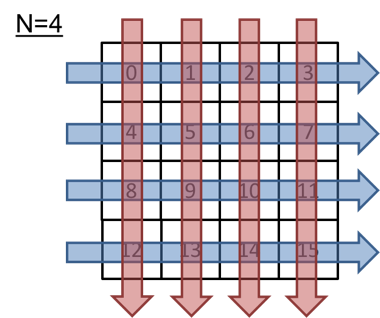
\includegraphics[width=0.5\textwidth,keepaspectratio,natwidth=193,natheight=40]
  {research/maruyama/lo02.png}
%  \caption{Calculation pattern of the benchmark program}
  \locallabel{fig:kmr-02}
\end{figure}

\begin{figure}
\centering
  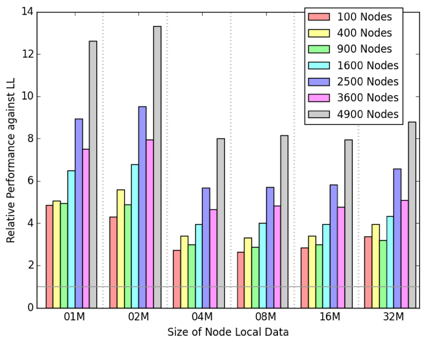
\includegraphics[width=0.5\textwidth,keepaspectratio,natwidth=193,natheight=40]
  {research/maruyama/lo03.png}
%  \caption{Experimental results}
  \locallabel{fig:kmr-03}
\end{figure}


\subsubsection{Skew-tuned shuffling for load balancing for Reduce operation}

In a MapReduce program, the number of tasks 


\subsubsection{Visualize MapReduce task execution}

\begin{figure}
\centering
  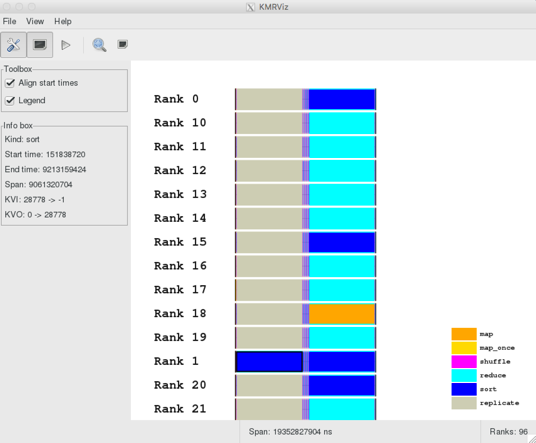
\includegraphics[width=0.5\textwidth,keepaspectratio,natwidth=193,natheight=40]
  {research/maruyama/kmrviz.png}
  \caption{Caption for a sample figure}
  \locallabel{fig:kmrviz}
\end{figure}


\subsubsection{Apache Spark on K computer}


\subsection{High Level Framework for High Performance AMR}
% Wahib

\subsection{High Performance Graph Analytics Study with Graph500}
% Maruyama

\section{Schedule and Future Plan}

\subsection{KMR}
% Takizawa & Matsuda

\subsection{High Level Framework for High Performance AMR}
% Wahib

\subsection{High Performance Graph Analytics Study with Graph500}
% Maruyama

%%% DO NOT EDIT BELOW

\section{Publications}

%\printbibliography[keyword=journal, heading=subbibliography, title={Journal Articles}, prefixnumbers={1-}, resetnumbers=true]
%\printbibliography[keyword=proceedings, heading=subbibliography, title={Conference Papers}, prefixnumbers={2-}, resetnumbers=true]
%\printbibliography[keyword=invited, heading=subbibliography, title={Invited Talks}, prefixnumbers={3-}, resetnumbers=true]
%\printbibliography[keyword=poster, heading=subbibliography, title={Posters and Presentations}, prefixnumbers={4-}, resetnumbers=true]
%\printbibliography[keyword=deliverable, heading=subbibliography, title={Patents and Deliverables}, prefixnumbers={5-}, resetnumbers=true]

\printbibliography[keyword=journal, heading=subbibliography, title={Journal Articles}, resetnumbers=true]
\printbibliography[keyword=proceedings, heading=subbibliography, title={Conference Papers}]
\printbibliography[keyword=invited, heading=subbibliography, title={Invited Talks}]
\printbibliography[keyword=poster, heading=subbibliography, title={Posters and Presentations}]
\printbibliography[keyword=deliverable, heading=subbibliography, title={Patents and Deliverables}]

\end{refsection}
